\documentclass{article}
\usepackage{graphicx, tikz-cd, float, titlepic, booktabs} % Required for inserting images
\usepackage{pgfplots}
\pgfplotsset{compat=1.15}
\usepackage{mathrsfs}
\usetikzlibrary{arrows}
\usepackage{amsmath, amssymb, amsthm, amsfonts, siunitx, physics, gensymb}
\AtBeginDocument{\RenewCommandCopy\qty\SI}
\usepackage[version=4]{mhchem}
\usepackage[most,many,breakable]{tcolorbox}
\usepackage{xcolor, fancyhdr, varwidth}
\usepackage[Glenn]{fncychap}
%Options: Sonny, Lenny, Glenn, Conny, Rejne, Bjarne, Bjornstrup
\usepackage{hyperref, cleveref}
\usepackage{icomma, enumitem} %comma as decimal and continue enumerate with [resume]
\usepackage{plimsoll} %use standard state symbol with \stst
\usepackage[danish]{babel}
%%%%%%%%%%%%%%%%%%%%%%%%%%%%%%
% SELF MADE COLORS
%%%%%%%%%%%%%%%%%%%%%%%%%%%%%%
\definecolor{myg}{RGB}{56, 140, 70}
\definecolor{myb}{RGB}{45, 111, 177}
\definecolor{myr}{RGB}{199, 68, 64}
\definecolor{mytheorembg}{HTML}{F2F2F9}
\definecolor{mytheoremfr}{HTML}{00007B}
\definecolor{mylenmabg}{HTML}{FFFAF8}
\definecolor{mylenmafr}{HTML}{983b0f}
\definecolor{mypropbg}{HTML}{f2fbfc}
\definecolor{mypropfr}{HTML}{191971}
\definecolor{myexamplebg}{HTML}{F2FBF8}
\definecolor{myexamplefr}{HTML}{88D6D1}
\definecolor{myexampleti}{HTML}{2A7F7F}
\definecolor{mydefinitbg}{HTML}{E5E5FF}
\definecolor{mydefinitfr}{HTML}{3F3FA3}
\definecolor{notesgreen}{RGB}{0,162,0}
\definecolor{myp}{RGB}{197, 92, 212}
\definecolor{mygr}{HTML}{2C3338}
\definecolor{myred}{RGB}{127,0,0}
\definecolor{myyellow}{RGB}{169,121,69}
\definecolor{myexercisebg}{HTML}{F2FBF8}
\definecolor{myexercisefg}{HTML}{88D6D1}
%%%%%%%%%%%%%%%%%%%%%%%%%%%%%%%%%%%%%%%%%%%%%%%%%%%%%%%%%%%%%%%%%%%%%%
% Box environments for theorems and problems
%%%%%%%%%%%%%%%%%%%%%%%%%%%%%%%%%%%%%%%%%%%%%%%%%%%%%%%%%%%%%%%%%%%%%
\setlength{\parindent}{1cm}
%================================
% Question BOX
%================================
\makeatletter
\newtcbtheorem{question}{Opgave}{enhanced,
	breakable,
	colback=white,
	colframe=myb!80!black,
	attach boxed title to top left={yshift*=-\tcboxedtitleheight},
	fonttitle=\bfseries,
	title={#2},
	boxed title size=title,
	boxed title style={%
			sharp corners,
			rounded corners=northwest,
			colback=tcbcolframe,
			boxrule=0pt,
		},
	underlay boxed title={%
			\path[fill=tcbcolframe] (title.south west)--(title.south east)
			to[out=0, in=180] ([xshift=5mm]title.east)--
			(title.center-|frame.east)
			[rounded corners=\kvtcb@arc] |-
			(frame.north) -| cycle;
		},
	#1
}{def}
\makeatother
%================================
% DEFINITION BOX
%================================

\newtcbtheorem[]{Definition}{Definition}{enhanced,
	before skip=2mm,after skip=2mm, colback=red!5,colframe=red!80!black,boxrule=0.5mm,
	attach boxed title to top left={xshift=1cm,yshift*=1mm-\tcboxedtitleheight}, varwidth boxed title*=-3cm,
	boxed title style={frame code={
					\path[fill=tcbcolback]
					([yshift=-1mm,xshift=-1mm]frame.north west)
					arc[start angle=0,end angle=180,radius=1mm]
					([yshift=-1mm,xshift=1mm]frame.north east)
					arc[start angle=180,end angle=0,radius=1mm];
					\path[left color=tcbcolback!60!black,right color=tcbcolback!60!black,
						middle color=tcbcolback!80!black]
					([xshift=-2mm]frame.north west) -- ([xshift=2mm]frame.north east)
					[rounded corners=1mm]-- ([xshift=1mm,yshift=-1mm]frame.north east)
					-- (frame.south east) -- (frame.south west)
					-- ([xshift=-1mm,yshift=-1mm]frame.north west)
					[sharp corners]-- cycle;
				},interior engine=empty,
		},
	fonttitle=\bfseries,
	title={#2},#1}{def}
\newtcbtheorem[]{definition}{Definition}{enhanced,
	before skip=2mm,after skip=2mm, colback=red!5,colframe=red!80!black,boxrule=0.5mm,
	attach boxed title to top left={xshift=1cm,yshift*=1mm-\tcboxedtitleheight}, varwidth boxed title*=-3cm,
	boxed title style={frame code={
					\path[fill=tcbcolback]
					([yshift=-1mm,xshift=-1mm]frame.north west)
					arc[start angle=0,end angle=180,radius=1mm]
					([yshift=-1mm,xshift=1mm]frame.north east)
					arc[start angle=180,end angle=0,radius=1mm];
					\path[left color=tcbcolback!60!black,right color=tcbcolback!60!black,
						middle color=tcbcolback!80!black]
					([xshift=-2mm]frame.north west) -- ([xshift=2mm]frame.north east)
					[rounded corners=1mm]-- ([xshift=1mm,yshift=-1mm]frame.north east)
					-- (frame.south east) -- (frame.south west)
					-- ([xshift=-1mm,yshift=-1mm]frame.north west)
					[sharp corners]-- cycle;
				},interior engine=empty,
		},
	fonttitle=\bfseries,
	title={#2},#1}{def}

\newtcbtheorem{theo}%
    {Theorem}{}{theorem}
\newtcolorbox{prob}[1]{colback=red!5!white,colframe=red!50!black,fonttitle=\bfseries,title={#1}}
%================================
% NOTE BOX
%================================

\usetikzlibrary{arrows,calc,shadows.blur}
\tcbuselibrary{skins}
\newtcolorbox{note}[1][]{%
	enhanced jigsaw,
	colback=gray!20!white,%
	colframe=gray!80!black,
	size=small,
	boxrule=1pt,
	title=\textbf{Note:},
	halign title=flush center,
	coltitle=black,
	breakable,
	drop shadow=black!50!white,
	attach boxed title to top left={xshift=1cm,yshift=-\tcboxedtitleheight/2,yshifttext=-\tcboxedtitleheight/2},
	minipage boxed title=1.5cm,
	boxed title style={%
			colback=white,
			size=fbox,
			boxrule=1pt,
			boxsep=2pt,
			underlay={%
					\coordinate (dotA) at ($(interior.west) + (-0.5pt,0)$);
					\coordinate (dotB) at ($(interior.east) + (0.5pt,0)$);
					\begin{scope}
						\clip (interior.north west) rectangle ([xshift=3ex]interior.east);
						\filldraw [white, blur shadow={shadow opacity=60, shadow yshift=-.75ex}, rounded corners=2pt] (interior.north west) rectangle (interior.south east);
					\end{scope}
					\begin{scope}[gray!80!black]
						\fill (dotA) circle (2pt);
						\fill (dotB) circle (2pt);
					\end{scope}
				},
		},
	#1,
}
%================================
% EXAMPLE BOX
%================================
\newtcbtheorem[number within=section]{Example}{Example}
{%
	colback = myexamplebg
	,breakable
	,colframe = myexamplefr
	,coltitle = myexampleti
	,boxrule = 1pt
	,sharp corners
	,detach title
	,before upper=\tcbtitle\par\smallskip
	,fonttitle = \bfseries
	,description font = \mdseries
	,separator sign none
	,description delimiters parenthesis
}
{ex}
%================================
% THEOREM BOX
%================================

\tcbuselibrary{theorems,skins,hooks}
\newtcbtheorem[number within=section]{Theorem}{Theorem}
{%
	enhanced,
	breakable,
	colback = mytheorembg,
	frame hidden,
	boxrule = 0sp,
	borderline west = {2pt}{0pt}{mytheoremfr},
	sharp corners,
	detach title,
	before upper = \tcbtitle\par\smallskip,
	coltitle = mytheoremfr,
	fonttitle = \bfseries\sffamily,
	description font = \mdseries,
	separator sign none,
	segmentation style={solid, mytheoremfr},
}
{th}

%%%%%%%%%%%%%%%%%%%%%%%%%%%%%%%%%%%%%%%%%%%%%%%%%%%%%%%%%%%%%%%%%
% SELF MADE COMMANDS
%%%%%%%%%%%%%%%%%%%%%%%%%%%%%%
\newcommand{\sol}{\setlength{\parindent}{0cm}\textbf{\textit{Løsning:}}\setlength{\parindent}{1cm}}
%%%%%%%%%%%%%%%%%%%%%%%%%%%%%%%%%
\usepackage[tmargin=2cm,rmargin=1in,lmargin=1in,margin=0.85in,bmargin=2cm,footskip=.2in]{geometry}\pagestyle{fancy}
\lhead{Minrui Kevin Zhou 3.b}
\rhead{Aflevering 36}

\title{Aflevering 36\\
{\Large \textbf{3.b mat A}}}
\author{Kevin Zhou}
\date{\today}

\begin{document}
\maketitle
\newpage
\begin{question}{}{}
  En funktion $f$ af to variable er givet ved
  \[
  f(x,y)= y^3+x^2+x \cdot y -4y
  \] 
  \begin{itemize}
    \item[a.] Undersøg, om gradienten $\grad f(1,2)$ og vektoren $\mqty(7\\ -3) $ er ortogonale. 
  \end{itemize}
\end{question}
\sol \\
\textbf{a.}
Vi beregner først et generelt udtryk for gradienten for $f$.
\begin{equation*}
\begin{split}
  \grad f(x,y)&=\mqty(\pdv{x} \left(y^3+x^2+x \cdot y -4y\right)\\ \pdv{y} \left(y^3+x^2+x \cdot y -4y\right)) \\
  &=\mqty(2x+y\\ 3y^2+x-4) 
\end{split}
\end{equation*}
Vi kan nu beregne $\grad f(1,2)$.
\begin{equation*}
\begin{split}
  \grad f(1,2)&=\mqty(2 \cdot 1 +2\\ 3 \cdot 2^2 + 1 -4) \\
  &=\mqty(4\\ 9) 
\end{split}
\end{equation*}
Siden to vektorer er ortogonale præcis når deres prikprodukt er 0, så beregner vi $\grad f(1,2) \cdot \mqty(7\\ -3) $.
\begin{equation*}
\begin{split}
  \grad f(1,2) \cdot \mqty(7\\ -3) &= \mqty(4\\ 9) \cdot \mqty(7\\ -3) \\
  &=4 \cdot 7 + 9 \cdot \left(-3\right) \\
  &=1 \\
  &\neq 0
\end{split}
\end{equation*}
Altså er de to vektorer ikke ortogonale.
\begin{question}{}{}
  En vektorfunktion $\va{s} $ er bestemt ved
  \[
  \va{s} (t)=\mqty(5+5 \cdot \cos\left(t\right) \\ 7+5 \cdot \sin\left(t\right) ), \quad 0 \leq t \leq 2 \pi 
  \] 
  Parameterkurven for $\va{s}$ er en cirkel.
  \begin{itemize}
    \item[a.] Bestem centrum og radius for cirklen.
  \end{itemize}
  Linjen $l$ er tangent til cirklen i punktet $P(8,11)$.
  \begin{itemize}
    \item[b.] Bestem en ligning for $l$.
  \end{itemize}
\end{question}
\sol \\
\textbf{a.}
Siden parameterfremstillingen for en cirkel med centrum i $\left(a,b\right) $ og radius $r$ er
\[
\mqty(x(t)\\ y(t))=\mqty(a + r \cdot \cos\left(t\right) \\ b + r \cdot \sin\left(t\right) ) 
\] 
så må den givne cirkel have centrum i $(5,7)$ og have radius $5$. \\[1ex]
\textbf{b.}
Vi finder først værdien af $t$, når $\va{s}(t)=\mqty(8\\ 11) $.
\begin{equation*}
\begin{split}
  \va{s}(t)=\mqty(8\\ 11) &\iff 5+5 \cdot \cos\left(t\right) =8 \land 7+5 \cdot \sin\left(t\right) =11\\
  &\implies t=\cos^{-1}\left(\frac{3}{5}\right) =\sin^{-1}\left(\frac{4}{5}\right) 
\end{split}
\end{equation*}
da $0 \leq t \leq 2 \pi $.
Vi finder nu forskriften for den afledede funktion for $\va{s} $.
\begin{equation*}
\begin{split}
  \va{s}'(t)&=\mqty(\dv{t} \left(5+5 \cdot \cos\left(t\right) \right) \\ \dv{t} \left(7+5 \cdot \sin\left(t\right) \right) ) \\
  &=\mqty(-5 \cdot \sin\left(t\right) \\ 5 \cdot \cos\left(t\right) ) 
\end{split}
\end{equation*}
Der gælder, at $\va{s}'(t)$ er retningsvektoren for tangenten til parameterkurven for $\va{s} $. 
Vi beregner nu $\va{s}'\left(\cos^{-1}\left(\frac{3}{5}\right) \right) $ (bemærk at $\cos^{-1}\left(\frac{3}{5}\right) =\sin^{-1}\left(\frac{4}{5}\right) $).
\begin{equation*}
\begin{split}
  \va{s}'\left(\cos^{-1}\left(\frac{3}{5}\right) \right) &=\mqty(-5 \cdot \sin\left(\sin^{-1}\left(\frac{4}{5}\right) \right) \\ 5 \cdot \cos\left(\cos^{-1}\left(\frac{3}{5}\right) \right) ) \\
  &=\mqty(-4\\ 3) 
\end{split}
\end{equation*}
Altså må en normalvektor til linjen $l$, der er tangent til cirklen i punktet $P(8,11)$ være $\va{n} =\mqty(3\\ 4) $, og en ligning for $l$ må da være 
\[
3 \cdot \left(x-8\right) +4 \cdot \left(y-11\right) =0
\] 
\begin{question}{}{}
  Den samlede biomasse af en population af helleflyndere i et område af Stillehavet kan beskrives ved modellen
$$\dfrac{dy}{dx}=0,71\cdot\Bigg(1-\dfrac{y}{80,5}\Bigg)\cdot y,$$
hvor $y=f(x)$ er populationens samlede biomasse (målt i mio. kg),
og $x$ er tiden (målt i år).
Til tidspunktet $x=0$ er den samlede biomasse 20,1 mio. kg.
\begin{itemize}
  \item[a.] Med hvilken hastighed vokser den samlede biomasse til tidspunktet $x=0?$
  \item[b.] Bestem et udtryk for den samlede biomasse $f(x).$
  \item[c.] Til hvilket tidspunkt når den samlede biomasse op på 75 mio. kg?
\end{itemize}
\end{question}
\sol \\
\textbf{a.}
Da der gælder, at $x=0 \implies y=20,1$, så må væksthastigheden være
\begin{equation*}
\begin{split}
  f'(20,1)&= 0,71 \cdot \left(1-\frac{20,1}{80,5}\right) \cdot 20,1\\
  &\approx 10,71
\end{split}
\end{equation*}
Altsår vokser den samlede biomasse med $10,71$ mio. kg per år til tidspunktet $x=0$. \\[1ex]
\textbf{b.}
Vi omskriver først differentialligningen.
\begin{equation*}
\begin{split}
  \dfrac{dy}{dx}=0,71\cdot\Bigg(1-\dfrac{y}{80,5}\Bigg)\cdot y \iff \dv{y}{x}=y \cdot \left(0,71-\frac{0,71}{80,5} \cdot y\right) 
\end{split}
\end{equation*}
Siden der for en ligning af formen
\[
y'=y(b-ay)
\] 
gælder, at den har de ikke-negative, voksende løsninger 
\[
g(x)= \frac{\frac{b}{a}}{1+c e^{-bx} }, \quad c \in \mathbb{R}^+, x \in \mathbb{R}
\] 
Altså må forskriften for $f$ være af formen 
\begin{equation*}
\begin{split}
  f(x)&= \frac{\frac{0,71 \cdot 80,5}{0,71}}{1+ c e^{-0,71x}  }\\
  &=\frac{80,5}{1+c e^{-0,71x} }
\end{split}
\end{equation*}
Siden $f(0)= 20,1$, så har vi 
\begin{equation*}
\begin{split}
  \frac{80,5}{1+c e^{-0,71 \cdot 0} }= 20,1 \iff c=\frac{80,5}{20,1}-1 \approx 3,005
\end{split}
\end{equation*}
Et udtryk for den samlede biomasse er altså
\[
f(x)= \frac{80,5}{1+\left(\frac{80,5}{20,1}-1\right) e^{-0,71x} } \approx \frac{80,5}{1+3,005 e^{-0,71x} }
\] 
En definitionsmængde, der giver mening er $Dm(f)=\mathbb{R}$. \\[1ex]
\noindent\textbf{c.}
Vi løser ligningen $f(x)= 75$.
\begin{equation*}
\begin{split}
  f(x)= 75 &\iff \frac{80,5}{1+\left(\frac{80,5}{20,1}-1\right) e^{-0,71x} }=75\\
  &\iff e^{-0,71x} \cdot \left(\frac{80,5}{20,1}-1\right)  =\frac{80,5}{75}-1\\
  &\iff e^{-0,71x} =\frac{80,5-75}{75 \cdot \left(\frac{80,5}{20,1}-1\right) }\\
  &\iff x=-\frac{\ln\left(\frac{80,5-75}{75 \cdot \left(\frac{80,5}{20,1}-1\right) }\right) }{0,71} \approx 5,23
\end{split}
\end{equation*}
Altså når den samlede biomasse op på $75$ mio. kg efter $5,23$ år. 

\begin{question}{}{}
  En funktion $f$ af to variable er givet ved

$$f(x,y)=x^2+y^2+2x.$$

Det oplyses, at $f$ har ét stationært punkt.
\begin{itemize}
  \item[a.] Bestem koordinatsættet til det stationære punkt
  \item[b.] Bestem arten af det stationære punkt.
\end{itemize}
\end{question}
\sol \\
\textbf{a.}
Vi finder først et udtryk for $\grad f(x,y)$.
\begin{equation*}
\begin{split}
  \grad f(x,y)&=\mqty(f'_x(x,y)\\ f'_y(x,y)) \\
  &=\mqty(2x+2\\ 2y) 
\end{split}
\end{equation*}
Ved det stationære punkt $(x_0,y_0)$ er gradienten $\grad f(x_0,y_0)=\mqty(0\\ 0)$. 
\begin{equation*}
\begin{split}
  \grad f(x_0,y_0)=\mqty(0\\ 0) &\iff \mqty(2x_0+2\\ 2y_0) =\mqty(0\\ 0) \\
  &\iff x_0=-1 \land y_0=0
\end{split}
\end{equation*}
Koordinatsættet til det stationære punkt er altså $(-1,0)$.\\[1ex]
\textbf{b.}
Vi beregner først den dobbelt partielle afledede af $f(x,y)$ mht. $x$ og $x$.
\begin{equation*}
\begin{split}
  f''_{xx}(x,y)&= \pdv{x} \left(f'_x(x,y)\right) \\
  &=\pdv{x} \left(2x+2\right) \\
  &=2
\end{split}
\end{equation*}
Vi beregner nu den dobbelt partielle afledede af $f(x,y)$ mht. $y$ og $y$.
\begin{equation*}
\begin{split}
  f''_{yy}(x,y)&= \pdv{y} \left(f'_y(x,y)\right) \\
  &=\pdv{y} \left(2y\right) \\
  &=2
\end{split}
\end{equation*}
Vi beregner nu den dobbelt partielle afledede af $f(x,y)$ mht. $x$ og $y$.
\begin{equation*}
\begin{split}
  f''_{xy}(x,y)&= \pdv{y} \left(f'_x(x,y)\right) \\
  &=\pdv{y} \left(2x\right) \\
  &=0
\end{split}
\end{equation*}
Vi ser da, at 
\begin{equation*}
\begin{split}
  f''_{xx}(-1,0) \cdot f''_{yy}(-1,0) - (f''_{xy}(-1,0))^2 &= 2 \cdot 2-0^2\\
  &=4 >0
\end{split}
\end{equation*}
Siden der også gælder, at 
\begin{equation*}
\begin{split}
  f''_{xx}(-1,0)=2>0
\end{split}
\end{equation*}
så må arten af det stationære punkt være et minimum.
\begin{question}{}{}
  Figuren viser grafen for funktionen $f$ givet ved
  \[
  f(x,y)= e^{1-(x^2-1)^2-y^2} 
  \] 
  Funktionen $f$ har tre stationære punkter $A$, $B$ og $C$. 
  \begin{itemize}
    \item[a.] Bestem koordinatsættet til hvert af punkterne $A$, $B$ og $C$. 
    \item[b.] Bestem længden af snitkurven fra punktet $A$ til punktet $B$. 
  \end{itemize}
\end{question}
\sol \\
\textbf{a.}
Vi finder først et udtryk for $\grad f(x,y)$ med kædereglen.
\begin{equation*}
\begin{split}
  \grad f(x,y)&=\mqty(\pdv{x} \left(e^{1-(x^2-1)^2-y^2} \right) \\ \pdv{y} \left(e^{1-(x^2-1)^2-y^2} \right) ) \\
  &=\mqty(e^{1-(x^2-1)^2-y^2} \cdot \left(4x-4x^3\right) \\ e^{1-(x^2-1)^2-y^2} \cdot 2y)\\
  &=\mqty(\left(4x-4x^3\right) \cdot e^{-x^4+2x^2-y^2} \\ 2y \cdot e^{-x^4+2x^2-y^2} ) 
\end{split}
\end{equation*}
Vi sætter denne lig $\mqty(0\\ 0) $ og finder løsningerne med CAS. 
\begin{equation*}
\begin{split}
  \grad f(x,y)= \mqty(\left(4x-4x^3\right) \cdot e^{-x^4+2x^2-y^2} \\ 2y \cdot e^{-x^4+2x^2-y^2} ) =\mqty(0\\ 0) \implies x=0 \land y=0
\end{split}
\end{equation*}
hvilket ikke kan være sandt, da der er tre stationære punkter.
Geo viser kun én løsning.
\begin{figure}[H]
\begin{center}
  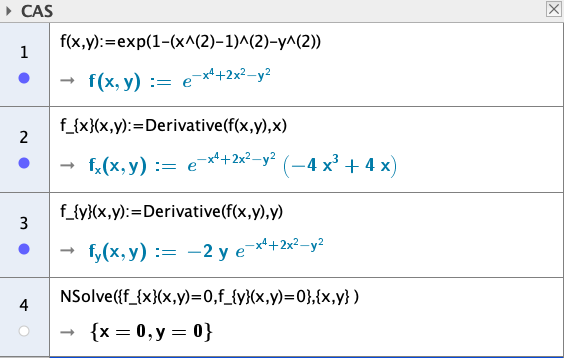
\includegraphics[width=\textwidth]{CAS.png}
\end{center}
\caption{GeoGebra viser kun én af løsningerne}
\label{fig:CAS}
\end{figure}

\end{document}
